\documentclass[8pt,a4paper]{beamer}
\usepackage[utf8]{inputenc}
\usepackage[spanish, es-tabla]{babel}
\usepackage{amsmath}
\usepackage{amsfonts}
\usepackage{amssymb}
\usepackage{graphicx}
\usepackage{extarrows} 
\usepackage{multirow}
\usepackage{ragged2e}
\usepackage{mathrsfs}
\usepackage{fancybox}
\usepackage{color}
\usepackage{multicol}
\usepackage{colortbl}

\usepackage{pifont} % Symbolos en las viñetas

%\setlength{\parskip}{1.5mm} %Espaciado

\setbeamertemplate{caption}[numbered]

\usetheme{Warsaw}
%\usecolortheme{crane}
%\usecolortheme{beaver}
%\usecolortheme{dolphin}
%\usecolortheme{seahorse}
%\usecolortheme{dove}

\usefonttheme[onlymath]{serif}

\titlegraphic{
\includegraphics[width=1.5cm]{logo.png}}
\author{Carlos Alberto Azula Díaz}
\title{\textsc{Pirámides de Población}}

\providecommand{\abs}[1]{\lvert#1\rvert}
\providecommand{\norm}[1]{\lVert#1\rVert}

\renewcommand{\familydefault}{\rmdefault}
%\renewcommand{\familydefault}{\sfdefault}

\setbeamercolor{structure}{fg=red!50!black}

\begin{document}

\frame{\titlepage}

\justifying{

\section{Pirámides de Población (Parte I)}
\subsection{1. Introducción}
\begin{frame}{\textbf{1. Introducción}}
\setlength{\parskip}{3px}
\justifying
Las pirámides de población son representaciones gráficas que nos permiten visualizar la distribución de edades y géneros en una población en un momento dado. Estas representaciones son una herramienta fundamental en la demografía, ya que nos brindan información valiosa sobre la estructura y las tendencias de una población. Al observar una pirámide de población, podemos analizar el crecimiento, el envejecimiento y otros aspectos demográficos que tienen impacto en la sociedad y la economía de un país o región.

En esta ocasión, exploraremos en detalle las pirámides de población, su definición, características y su importancia como instrumento demográfico. Analizaremos los diferentes tipos de pirámides de población, como las expansivas, estables o estacionarias, y regresivas o envejecidas, y discutiremos las implicaciones demográficas y sociales asociadas a cada tipo. Además, exploraremos la interpretación de las pirámides de población y cómo podemos utilizarlas para la planificación y formulación de políticas públicas.

También examinaremos cómo las pirámides de población cambian a lo largo del tiempo y los factores que influyen en su evolución, como la natalidad, la mortalidad y la migración. A través de ejemplos históricos y proyecciones futuras, podremos comprender mejor los posibles escenarios demográficos y su impacto en distintas sociedades.

\end{frame}

\begin{frame}{}
\setlength{\parskip}{3px}
\justifying
El objetivo principal de esta exposición es destacar la importancia de comprender y analizar las pirámides de población como una herramienta esencial para la toma de decisiones informadas en ámbitos como la planificación urbana, la educación, la salud y la seguridad social. Asimismo, se espera despertar el interés por profundizar en este tema y explorar posibles líneas de investigación futuras.

A lo largo de este análisis, nos adentraremos en el fascinante mundo de las pirámides de población y descubriremos cómo estas representaciones gráficas pueden revelar información clave sobre una población, su dinámica y su evolución en el tiempo. ¡Comencemos a explorar las pirámides de población y desvelar sus secretos demográficos!
\end{frame}

\begin{frame}{}
\begin{block}{\textbf{1.1. Breve explicación del concepto de pirámides de población}}
\setlength{\parskip}{3px}
\justifying
Las pirámides de población son representaciones gráficas que muestran la distribución de edades y géneros en una población en un momento determinado. Toman su nombre de su forma característica, que se asemeja a una pirámide con una base ancha y puntas estrechas. En el eje vertical se representa la edad, dividida en grupos quinquenales o decenales, y en el eje horizontal se muestra la proporción o el número de personas en cada grupo de edad.

Las pirámides de población suelen estar compuestas por barras que representan a cada grupo de edad y se dividen en dos colores o secciones, una para hombres y otra para mujeres. La longitud de cada barra indica la cantidad de personas en ese grupo de edad y sexo específico. Por lo tanto, al observar una pirámide de población, podemos visualizar fácilmente la estructura y la composición demográfica de una población, así como detectar patrones y tendencias importantes.

Estas representaciones son una herramienta fundamental en la demografía, ya que nos permiten analizar aspectos clave como el crecimiento demográfico, la distribución por género, la esperanza de vida, el envejecimiento de la población, entre otros. Además, las pirámides de población también pueden proporcionar información valiosa sobre las necesidades y los desafíos socioeconómicos de una sociedad, ya que la estructura demográfica influye en áreas como la educación, la salud, la economía y la planificación urbana.

\end{block}
\end{frame}

\begin{frame}{}
\begin{block}{}
\justifying
En resumen, las pirámides de población son gráficos que nos ayudan a visualizar la distribución de edades y géneros en una población en un momento dado. Son una herramienta esencial para comprender la estructura demográfica de una sociedad, así como para analizar las tendencias y los desafíos asociados con el crecimiento y el envejecimiento de la población.
\end{block}

\end{frame}

\begin{frame}{}
\begin{block}{\textbf{1.2. Importancia de las pirámides de población como herramienta demográfica}}
Las pirámides de población son una herramienta demográfica de gran importancia debido a las siguientes razones:
\begin{enumerate}
\justifying
\item[1.] \textbf{Visualización de la estructura demográfica:} Las pirámides de población permiten una representación gráfica clara y concisa de la distribución de edades y géneros en una población en un momento dado. Esto facilita la comprensión de la estructura demográfica de una sociedad, mostrando la proporción de jóvenes, adultos y personas mayores, así como las diferencias en la distribución por género.

\item[2.] \textbf{Identificación de patrones y tendencias demográficas:} Al analizar las formas y características de las pirámides de población, es posible identificar patrones y tendencias demográficas importantes. Por ejemplo, una pirámide con una base ancha indica una alta tasa de natalidad y una población joven, mientras que una forma más rectangular o con una parte superior más amplia indica una población más envejecida. Estas tendencias demográficas tienen implicaciones significativas en áreas como la salud, la educación, la economía y la planificación urbana.

\item[3.] \textbf{Evaluación del crecimiento y envejecimiento de la población:} Las pirámides de población permiten evaluar el crecimiento demográfico y el envejecimiento de una población. 
\end{enumerate}
\end{block}
\end{frame}

\begin{frame}{}
\begin{block}{}
\begin{enumerate}
\justifying
\item[{}] Al comparar las pirámides de diferentes momentos en el tiempo, es posible identificar cambios en la estructura demográfica y determinar si la población está creciendo, disminuyendo o envejeciendo. Esto proporciona información esencial para la planificación y formulación de políticas en áreas como la atención médica, la seguridad social y la educación.

\item[4.] \textbf{Estimación de necesidades y desafíos sociales:} Al analizar las pirámides de población, se pueden inferir las necesidades y desafíos socioeconómicos de una sociedad. Por ejemplo, una pirámide con una proporción significativa de jóvenes puede indicar una mayor demanda de servicios educativos y de atención médica pediátrica. Del mismo modo, una pirámide con una población envejecida puede señalar la necesidad de políticas y programas dirigidos a la atención de la salud y el bienestar de las personas mayores.

\item[5.] \textbf{Planificación y toma de decisiones informadas:} Las pirámides de población proporcionan datos demográficos clave que ayudan en la planificación y toma de decisiones informadas a nivel gubernamental, organizacional y comunitario. Los responsables de formular políticas pueden utilizar esta información para diseñar estrategias de desarrollo, asignar recursos de manera adecuada y abordar los desafíos demográficos específicos de una población.

\end{enumerate}
\end{block}
\end{frame}

\begin{frame}{}
\justifying
\begin{block}{}
\justifying
En resumen, las pirámides de población son una herramienta demográfica esencial que nos permite comprender la estructura, las tendencias y los desafíos de una población. Su importancia radica en su capacidad para visualizar la distribución de edades y géneros, identificar patrones demográficos, evaluar el crecimiento y envejecimiento de la población, estimar necesidades y desafíos sociales, y respaldar la planificación y toma de decisiones informadas.
\end{block}

\end{frame}

\begin{frame}{}
\begin{block}{\textbf{1.3. Presentación de los objetivos del tema}}
\justifying
En esta sección, presentaremos los objetivos del tema de las pirámides de población. Estos objetivos establecen las metas que deseamos alcanzar al explorar este tema demográfico. A continuación, se presentan los principales objetivos:
\begin{enumerate}
\justifying
\item[1.] \textbf{Comprender el concepto y la importancia de las pirámides de población:} El primer objetivo es adquirir una comprensión clara del concepto de las pirámides de población y su relevancia como herramienta demográfica. Exploraremos cómo estas representaciones gráficas nos ayudan a visualizar la estructura demográfica de una población y a identificar patrones y tendencias importantes.

\item[2.] \textbf{Analizar los diferentes tipos de pirámides de población:} El segundo objetivo consiste en analizar en detalle los diferentes tipos de pirámides de población. Estudiaremos las características y peculiaridades de las pirámides expansivas, estables o estacionarias, y regresivas o envejecidas. Además, examinaremos las implicaciones demográficas y sociales asociadas con cada tipo de pirámide.

\item[3.] \textbf{Interpretar las pirámides de población y su relación con indicadores socioeconómicos:} El tercer objetivo es desarrollar habilidades para interpretar las pirámides de población y comprender su relación con los indicadores socioeconómicos. 

\end{enumerate}
\end{block}

\end{frame}


\begin{frame}{}
\begin{block}{}
\justifying

\begin{enumerate}
\justifying
\item[{}] Analizaremos cómo la forma y las variaciones en las pirámides de población pueden reflejar aspectos como el crecimiento demográfico, el envejecimiento de la población y las disparidades de género, entre otros.

\item[4.] Explorar los cambios en las pirámides de población a lo largo del tiempo: El cuarto objetivo se centra en examinar cómo las pirámides de población cambian a lo largo del tiempo. Estudiaremos los factores demográficos que influyen en la evolución de las pirámides, como la natalidad, la mortalidad y la migración. También exploraremos ejemplos históricos de cambios significativos en las pirámides de población y consideraremos las proyecciones futuras y posibles escenarios demográficos.

\item[5.] Reconocer la utilidad de las pirámides de población en la planificación y políticas públicas: El último objetivo es comprender la utilidad práctica de las pirámides de población en la planificación y formulación de políticas públicas. Analizaremos cómo estas herramientas demográficas pueden ayudar a abordar desafíos sociales y respaldar la toma de decisiones informadas en áreas como la salud, la educación, la economía y la planificación urbana.
\end{enumerate}
Al lograr estos objetivos, obtendremos una comprensión sólida de las pirámides de población como herramienta demográfica y podremos utilizar esta información para analizar y abordar los desafíos y oportunidades que surgen en el contexto de las dinámicas poblacionales.
\end{block}

\end{frame}


\subsection{2. Definición y características de las pirámides de población}
\begin{frame}{\textbf{2. Definición y características de las pirámides de población}}
\begin{block}{\textbf{2.1. Explicación detallada de qué son las pirámides de población:}}
\justifying
Las pirámides de población son representaciones gráficas que nos permiten visualizar la distribución de edades y géneros en una población en un momento específico. Estas representaciones toman su nombre de su forma característica, que se asemeja a una pirámide con una base ancha y puntas estrechas. En esencia, las pirámides de población muestran la composición demográfica de una población en función de las diferentes cohortes de edad y el número de personas en cada grupo.

En una pirámide de población, el eje vertical representa la edad y se divide generalmente en grupos quinquenales o decenales, mientras que el eje horizontal muestra la proporción o el número de personas en cada grupo de edad. Las barras que conforman la pirámide representan a cada grupo de edad y se dividen en dos colores o secciones, una para hombres y otra para mujeres. La longitud de cada barra indica la cantidad de personas en ese grupo de edad y sexo específico.

La información proporcionada por las pirámides de población puede ser muy útil para comprender la estructura demográfica de una población y obtener información valiosa sobre su dinámica. Al observar una pirámide de población, se pueden extraer varios datos demográficos clave, como el tamaño de la población en cada grupo de edad, la proporción de hombres y mujeres en cada grupo, la concentración de población joven o anciana, y las diferencias entre los grupos de edad.

\end{block}
\end{frame}

\begin{frame}{}
\begin{block}{}
\justifying
Las pirámides de población permiten identificar y analizar diferentes patrones demográficos. Por ejemplo, una base ancha en la pirámide indica una alta tasa de natalidad y una población joven, mientras que una base más estrecha puede indicar una disminución en la tasa de natalidad. Además, una parte superior más amplia de la pirámide puede señalar una población más envejecida, lo que implica una mayor proporción de personas mayores.

Estos patrones y tendencias demográficas tienen importantes implicaciones sociales, económicas y políticas. Por ejemplo, una población joven puede requerir mayores inversiones en educación y atención médica pediátrica, así como políticas de planificación familiar. Por otro lado, una población envejecida puede implicar desafíos en términos de atención médica, seguridad social y planificación para el cuidado de las personas mayores.

Además, las pirámides de población son útiles para realizar comparaciones entre diferentes poblaciones, regiones o países. Al analizar pirámides de población de diferentes lugares, se pueden identificar variaciones en la estructura demográfica y comprender las diferencias en términos de crecimiento, envejecimiento y distribución por género.

\end{block}

\end{frame}

\begin{frame}{}
\begin{block}{}
\justifying

En resumen, las pirámides de población son herramientas gráficas que nos permiten visualizar la distribución de edades y géneros en una población en un momento determinado. Estas representaciones proporcionan información valiosa sobre la estructura demográfica, los patrones de crecimiento y envejecimiento, y las diferencias entre grupos de edad en una población. Su análisis ayuda a comprender la dinámica demográfica y es fundamental para la planificación y formulación de políticas en diversas áreas socioeconómicas.
\end{block}
\end{frame}

\begin{frame}{}
\begin{block}{\textbf{2.2. Descripción de los elementos y datos que se representan en una pirámide de población}}
\justifying
Una pirámide de población muestra la distribución de edades y géneros en una población específica en un momento determinado. Para comprender mejor los elementos y datos que se representan en una pirámide de población, consideremos los siguientes aspectos:
\begin{enumerate}
\justifying
\item[1.] \textbf{Eje vertical (eje de edad):} El eje vertical de la pirámide de población representa la edad de la población y se divide generalmente en grupos quinquenales o decenales. Cada grupo de edad se muestra en forma de barras horizontales que van desde la base hasta la cúspide de la pirámide.

\item[2.] \textbf{Eje horizontal (eje de cantidad de población):} El eje horizontal representa la cantidad de población en cada grupo de edad. Puede estar representado en números absolutos o en porcentajes, dependiendo de la representación gráfica utilizada. Este eje permite comparar visualmente la cantidad de personas en diferentes grupos de edad.

\item[3.] \textbf{Barras de diferentes longitudes:} Cada grupo de edad está representado por una barra horizontal en la pirámide. La longitud de cada barra representa la cantidad de personas en ese grupo de edad. Las barras son de diferentes longitudes para cada grupo de edad, lo que permite visualizar la distribución de la población en función de la edad.
\end{enumerate}
\end{block}
\end{frame}

\begin{frame}{}
\begin{block}{}
\justifying
\begin{enumerate}
\justifying
\item[4.] \textbf{Divisiones por género:} Las pirámides de población suelen tener divisiones por género. En la representación gráfica, se utilizan diferentes colores o secciones para distinguir entre hombres y mujeres. Esto permite observar las diferencias en la distribución de edades entre los sexos y comprender la estructura de la población por género.

\item[5.] \textbf{Forma y estructura de la pirámide:} La forma y la estructura de la pirámide proporcionan información adicional sobre la composición demográfica de una población. Por ejemplo, una pirámide con una base ancha y puntas estrechas indica una alta tasa de natalidad y una población joven. En contraste, una pirámide con una base estrecha y una parte superior más amplia sugiere una población envejecida.
\end{enumerate}
Además de estos elementos visuales, los datos específicos que se pueden obtener de una pirámide de población incluyen:
\begin{itemize}
\justifying
\item[\ding{65}] \textbf{Tamaño de la población en cada grupo de edad:} Al observar las barras de la pirámide, se puede determinar cuántas personas hay en cada grupo de edad específico.
\end{itemize}
\end{block}
\end{frame}

\begin{frame}{}
\begin{block}{}
\justifying
\begin{itemize}
\justifying
\item[\ding{65}] \textbf{Proporción de género en cada grupo de edad:} Las divisiones por género en la pirámide permiten comparar la cantidad de hombres y mujeres en diferentes grupos de edad y entender las diferencias demográficas por sexo.
\item[\ding{65}] \textbf{Relación entre grupos de edad:} La comparación de las longitudes de las barras en diferentes grupos de edad permite analizar la relación entre grupos específicos. Por ejemplo, se pueden identificar los grupos de edad más grandes y más pequeños, así como la distribución de la población en diferentes etapas de la vida.
\end{itemize}
En resumen, una pirámide de población representa visualmente la distribución de edades y géneros en una población. Los elementos clave que se representan incluyen el eje vertical de edad, el eje horizontal de cantidad de población, las barras de diferentes longitudes para cada grupo de edad, las divisiones por género y la forma general de la pirámide. A partir de estos elementos, se pueden obtener datos como el tamaño de la población en cada grupo de edad, la proporción de género en cada grupo, y la relación entre los diferentes grupos de edad. Estos datos proporcionan una visión detallada de la estructura demográfica de una población y permiten analizar patrones, tendencias y disparidades demográficas. La interpretación de estos datos es fundamental para comprender la dinámica demográfica y abordar los desafíos y oportunidades asociados con la composición de la población en términos de edad y género.
\end{block}
\end{frame}


\begin{frame}{}
\begin{block}{\textbf{2.3. Enumeración de las características comunes de las pirámides de población (forma, simetría, variaciones)}}
\justifying
Las pirámides de población pueden presentar diversas características que reflejan la estructura demográfica de una población en un momento determinado. A continuación se enumeran algunas de las características comunes de las pirámides de población:
\begin{enumerate}
\justifying
\item[1.] \textbf{Forma:} La forma de una pirámide de población se refiere a su apariencia general. Puede variar desde una forma de "pirámide clásica" con una base ancha y puntas estrechas, hasta formas más irregulares o atípicas. La forma está determinada por los patrones de natalidad, mortalidad y migración en la población.

\item[2.] \textbf{Simetría:} La simetría en una pirámide de población se refiere a la igualdad o equilibrio en la distribución de edades y géneros. Una pirámide simétrica muestra una distribución relativamente uniforme de la población en todos los grupos de edad y una proporción similar de hombres y mujeres en cada grupo. Sin embargo, en la práctica, es poco común encontrar pirámides totalmente simétricas.
\end{enumerate}
\end{block}
\end{frame}

\begin{frame}{}
\justifying
\begin{block}{}
\justifying
\begin{enumerate}
\justifying
\item[3.] \textbf{Variaciones en la forma:} Las pirámides de población pueden variar en su forma según las características demográficas de una población en particular. Algunas variaciones comunes incluyen:
\begin{itemize}
\justifying
\item[a)] \textbf{Pirámides expansivas:} Estas pirámides tienen una base ancha, lo que indica una alta tasa de natalidad y una población joven en crecimiento. A medida que se avanza en las cohortes de edad, las barras se vuelven más estrechas, lo que refleja una disminución gradual de la población debido a la mortalidad.

\item[b)] \textbf{Pirámides estables o estacionarias:} Estas pirámides tienen una forma más rectangular, con una distribución equilibrada de la población en los diferentes grupos de edad. Indican una estabilidad en la estructura demográfica con tasas de natalidad y mortalidad relativamente constantes.

\item[c)] \textbf{Pirámides regresivas o envejecidas:} Estas pirámides tienen una base estrecha y una parte superior más amplia, lo que indica una baja tasa de natalidad y una población envejecida. La proporción de personas mayores es mayor que la de personas jóvenes, lo que puede tener implicaciones para los sistemas de atención médica y las políticas de seguridad social.
\end{itemize}

\item[4.] \textbf{Variaciones en la distribución por género:} Además de la distribución por edad, las pirámides de población también pueden mostrar las diferencias entre hombres y mujeres en cada grupo de edad. Estas diferencias pueden reflejar patrones culturales, sociales y biológicos, y pueden tener implicaciones en términos de equidad de género y necesidades específicas de cada grupo.
\end{enumerate}
\end{block}
\end{frame}


\begin{frame}{}
\justifying
\begin{block}{}
\justifying
Es importante destacar que las características de las pirámides de población pueden variar según el contexto geográfico, cultural y socioeconómico. Por lo tanto, es fundamental analizar las pirámides de población en conjunto con otros datos demográficos y considerar el contexto específico para obtener una comprensión completa de la estructura y las dinámicas demográficas de una población.
\end{block}
\end{frame}

\subsection{3. Tipos de pirámides de población}
\begin{frame}{\textbf{3. Tipos de pirámides de población}}
\begin{block}{\textbf{3.1. Pirámides de población expansivas}}
\justifying
\begin{enumerate}
\justifying
\item[A.] \textbf{Descripción de sus características principales}:  Las pirámides de población expansivas son aquellas que presentan una base ancha y puntas estrechas, lo que indica una alta tasa de natalidad y un crecimiento demográfico significativo en la población. Estas pirámides son típicas de las sociedades donde las tasas de natalidad son altas y la esperanza de vida es relativamente corta.

Las características principales de las pirámides de población expansivas son las siguientes:
\begin{itemize}
\justifying
\item[\ding{65}] \textbf{Base ancha:} La base ancha de la pirámide representa una gran cantidad de personas en los grupos de edad más jóvenes, como los niños y los adolescentes. Esta amplia base indica una alta tasa de natalidad y un gran número de nacimientos en la población.

\item[\ding{65}] \textbf{Disminución gradual en las cohortes de edad:} A medida que se avanza en los grupos de edad, las barras de la pirámide se vuelven más estrechas. Esto refleja una disminución gradual en la cantidad de personas a medida que se produce un aumento en las tasas de mortalidad.

\item[\ding{65}]  \textbf{Proporción equilibrada de género:} En las pirámides de población expansivas, generalmente se observa una proporción equilibrada entre hombres y mujeres en cada grupo de edad. Esto indica que la alta tasa de natalidad se aplica tanto a hombres como a mujeres.
\end{itemize}

\end{enumerate}
\end{block}
\end{frame}

\begin{frame}{}
\begin{block}{}
\begin{enumerate}
\justifying
\item[{}] 
\begin{itemize}
\justifying
\item[\ding{65}] \textbf{Ausencia de una parte superior amplia:} En las pirámides de población expansivas, la parte superior de la pirámide tiende a ser más estrecha que la base. Esto se debe a que la mortalidad es más alta en las edades más avanzadas y la esperanza de vida es relativamente corta en comparación con las tasas de natalidad.

\item[\ding{65}] \textbf{Alto crecimiento demográfico:} La presencia de una base ancha en la pirámide de población expansiva indica un alto crecimiento demográfico en la población. Esto se debe a que hay una gran cantidad de personas en edad reproductiva que están dando a luz a una gran cantidad de hijos.
\end{itemize}
Las pirámides de población expansivas suelen ser características de países en desarrollo o en transición demográfica, donde las tasas de natalidad son altas y la esperanza de vida está aumentando gradualmente. Estas pirámides reflejan una población joven y en crecimiento, lo que puede tener implicaciones para la planificación y el desarrollo social, económico y de salud en esos países.
\item[B.] \textbf{Ejemplos de países o regiones con pirámides de este tipo:} Las pirámides de población expansivas son comunes en países o regiones con altas tasas de natalidad y un crecimiento demográfico significativo. Algunos ejemplos de países o regiones que han mostrado pirámides de población expansivas en el pasado incluyen:
\end{enumerate}
\end{block}
\end{frame}

\begin{frame}{}
\begin{block}{}
\justifying
\begin{enumerate}
\justifying
\item[{}]
\begin{enumerate}
\justifying
\item[1)] \textbf{Países en desarrollo de África subsahariana:} Varios países en África subsahariana han experimentado pirámides de población expansivas debido a sus altas tasas de natalidad. Por ejemplo, Níger, Malí, Uganda y República Democrática del Congo han mostrado pirámides de población expansivas en años anteriores.

\item[2)] \textbf{Países del Medio Oriente y del Norte de África:} Algunos países de esta región también han presentado pirámides de población expansivas. Por ejemplo, Yemen, Arabia Saudita y Egipto han tenido pirámides de población con bases anchas en el pasado, indicando altas tasas de natalidad.

\item[3)] \textbf{Países en desarrollo de Asia:} En el pasado, países como India, Pakistán y Bangladesh han mostrado pirámides de población expansivas debido a sus altas tasas de natalidad y grandes poblaciones jóvenes.
\end{enumerate}
Es importante tener en cuenta que las pirámides de población pueden cambiar con el tiempo debido a factores como cambios en las tasas de natalidad, mortalidad y migración. Por lo tanto, es posible que algunos de los países mencionados hayan experimentado cambios en sus pirámides de población en los últimos años debido a las transiciones demográficas y cambios en las políticas de planificación familiar.

Además, es fundamental tener en cuenta que los patrones demográficos pueden variar dentro de un país o región, por lo que es posible que se observen diferencias en las pirámides de población entre diferentes áreas geográficas dentro del mismo país.
\end{enumerate}
\end{block}
\end{frame}

\begin{frame}{}
\begin{block}{}
\justifying
\begin{enumerate}
\justifying
\item[C.] \textbf{Explicación de las implicaciones demográficas y sociales de una pirámide expansiva:} Una pirámide de población expansiva, caracterizada por una base amplia y puntas estrechas, tiene varias implicaciones demográficas y sociales. Estas implicaciones se derivan de las altas tasas de natalidad y el crecimiento demográfico significativo que refleja la pirámide. A continuación, se explican algunas de las implicaciones más destacadas:
\begin{enumerate}
\justifying
\item[1)] \textbf{Demográficas:} 
\begin{itemize}
\justifying
\item[\ding{65}] \textbf{Crecimiento poblacional acelerado:} La presencia de una base amplia en la pirámide indica que hay una gran cantidad de personas en edad reproductiva. Esto, a su vez, se traduce en un alto número de nacimientos y un crecimiento demográfico acelerado en la población. Esto puede tener implicaciones en la demanda de servicios básicos, como salud, educación, vivienda y empleo.

\item[\ding{65}] \textbf{Presión sobre los recursos naturales:} Un alto crecimiento demográfico puede ejercer presión sobre los recursos naturales, como tierra cultivable, agua, energía y alimentos. Esto puede resultar en problemas de escasez, degradación ambiental y desafíos para la sostenibilidad y la planificación adecuada del desarrollo.

\item[\ding{65}] \textbf{Cambios en la estructura de edad:} A medida que la población joven de la base de la pirámide se desplaza hacia las cohortes de edad más avanzadas, se esperan cambios en la estructura de edad. Esto puede generar desafíos relacionados con el envejecimiento de la población en el futuro, como el aumento de la demanda de atención médica, el sistema de pensiones y la atención a largo plazo.
\end{itemize}
\end{enumerate}
\end{enumerate}
\end{block}
\end{frame}


\begin{frame}{}
\begin{block}{}
\justifying
\begin{enumerate}
\justifying
\item[{}] 
\begin{enumerate}
\justifying
\item[2)] \textbf{Sociales:} 
\begin{itemize}
\justifying
\item[\ding{65}] \textbf{Presión sobre los servicios sociales:} Un alto crecimiento demográfico puede poner presión sobre los servicios sociales, como la educación y la atención médica. La necesidad de infraestructuras educativas y sanitarias adecuadas para una población joven y en crecimiento puede ser un desafío para los sistemas de salud y educación.

\item[\ding{65}] \textbf{Desafíos en la planificación familiar:} La presencia de una pirámide de población expansiva puede señalar la necesidad de programas y políticas de planificación familiar efectivos. Es importante garantizar el acceso a métodos anticonceptivos y educación sexual, así como promover la toma de decisiones informadas sobre el tamaño de la familia.

\item[\ding{65}] \textbf{Oportunidades demográficas:} Una pirámide de población expansiva también puede indicar una gran población joven en edad laboral. Si se aprovechan adecuadamente, estas cohortes de edad pueden brindar oportunidades para el desarrollo económico, la fuerza laboral productiva y la innovación.
\end{itemize}
\end{enumerate}
Es crucial tener en cuenta que las implicaciones demográficas y sociales pueden variar según el contexto político, socioeconómico y cultural de un país o región. Además, las políticas y programas adecuados pueden ayudar a abordar los desafíos y aprovechar las oportunidades asociadas con una pirámide de población expansiva, promoviendo un desarrollo sostenible y una mejora en la calidad de vida de la población.
\end{enumerate}
\end{block}
\end{frame}

\begin{frame}{}
\begin{block}{\textbf{3.2. Pirámides de población estables o estacionarias}}
\justifying
\begin{enumerate}
\justifying
\item[A.] \textbf{Descripción de sus características principales}:  Las pirámides de población estables o estacionarias son aquellas en las que la distribución de la población en los diferentes grupos de edad muestra un equilibrio relativo y una forma rectangular. Estas pirámides reflejan una estabilidad demográfica a lo largo del tiempo, con tasas de natalidad y mortalidad relativamente constantes.

Las características principales de las pirámides de población estables o estacionarias son las siguientes:
\begin{itemize}
\justifying
\item[\ding{65}] \textbf{Forma rectangular:} A diferencia de las pirámides de población expansivas o regresivas, las pirámides estables tienen una forma rectangular, con una distribución equilibrada de la población en los diferentes grupos de edad. Esto indica una proporción similar de personas en cada cohorte de edad, desde los niños hasta los ancianos.

\item[\ding{65}] \textbf{Cohortes de edad similares:} En las pirámides de población estables, las barras de la pirámide suelen tener una altura relativamente constante en la mayoría de los grupos de edad. Esto sugiere que las tasas de natalidad y mortalidad son similares en cada cohorte de edad, lo que contribuye a una distribución estable de la población.

\item[\ding{65}]  \textbf{Equilibrio de género:} En general, las pirámides estables muestran una proporción equilibrada de hombres y mujeres en cada grupo de edad. Esto significa que no hay una predominancia significativa de un género sobre el otro en ninguna cohorte de edad.
\end{itemize}

\end{enumerate}
\end{block}
\end{frame}

\begin{frame}{}
\begin{block}{}
\begin{enumerate}
\justifying
\item[{}] 
\begin{itemize}
\justifying
\item[\ding{65}] \textbf{Estabilidad demográfica:} Las pirámides de población estables indican una estabilidad demográfica a lo largo del tiempo, con tasas de natalidad y mortalidad relativamente constantes. Esto puede ser el resultado de un equilibrio entre la cantidad de nacimientos y la cantidad de defunciones en la población.

\item[\ding{65}] \textbf{Expectativa de vida promedio similar en diferentes cohortes:} Dado que las pirámides estables reflejan tasas de mortalidad constantes en diferentes grupos de edad, es probable que la expectativa de vida promedio sea similar en la mayoría de las cohortes. Esto implica que no hay una brecha significativa en la esperanza de vida entre los jóvenes y los ancianos.
\end{itemize}
Las pirámides de población estables o estacionarias son características de las sociedades en las que las tasas de natalidad y mortalidad se mantienen relativamente constantes durante un período prolongado. Estas pirámides reflejan una distribución equilibrada de la población por edad y género, lo que puede tener implicaciones en áreas como la planificación de servicios sociales, la fuerza laboral y la planificación económica a largo plazo.
\item[B.] \textbf{Ejemplos de países o regiones con pirámides de este tipo:} Las pirámides de población estables o estacionarias pueden encontrarse en países o regiones donde las tasas de natalidad y mortalidad se han mantenido relativamente constantes durante un período prolongado. Algunos ejemplos de países o regiones que han mostrado pirámides de población estables en el pasado o en la actualidad incluyen:
\end{enumerate}
\end{block}
\end{frame}

\begin{frame}{}
\begin{block}{}
\justifying
\begin{enumerate}
\justifying
\item[{}]
\begin{enumerate}
\justifying
\item[1)] \textbf{Países desarrollados de Europa:} Varios países europeos, como Alemania, Francia, España y Suecia, han tenido pirámides de población estables en los últimos años. Estos países han experimentado una disminución en las tasas de natalidad y mortalidad, lo que ha resultado en una estructura de edad relativamente equilibrada.

\item[2)] \textbf{Japón:} Japón es conocido por tener una pirámide de población estable y, en algunos casos, incluso invertida debido a su baja tasa de natalidad y una esperanza de vida alta. Esta estructura demográfica ha llevado a desafíos relacionados con el envejecimiento de la población y la sostenibilidad del sistema de pensiones.

\item[3)] \textbf{Canadá y Australia:} Estos países han experimentado una estabilidad demográfica en términos de tasas de natalidad y mortalidad, lo que ha resultado en pirámides de población relativamente estables en las últimas décadas.
\end{enumerate}
Es importante tener en cuenta que las pirámides de población pueden cambiar con el tiempo debido a diversos factores, como cambios en las políticas de inmigración, planificación familiar y salud pública. Además, las características específicas de las pirámides de población pueden variar dentro de un país, especialmente en países grandes y diversos, donde pueden existir diferencias regionales en términos de estructura demográfica.
\end{enumerate}
\end{block}
\end{frame}

\begin{frame}{}
\begin{block}{}
\justifying
\begin{enumerate}
\justifying
\item[C.] \textbf{Explicación de las implicaciones demográficas y sociales de una pirámide estable:} Una pirámide de población estable, caracterizada por una distribución equilibrada de la población en los diferentes grupos de edad, tiene varias implicaciones demográficas y sociales. Estas implicaciones se derivan de las tasas de natalidad y mortalidad relativamente constantes que refleja la pirámide. A continuación, se explican algunas de las implicaciones más destacadas:
\begin{enumerate}
\justifying
\item[1)] \textbf{Demográficas:} 
\begin{itemize}
\justifying
\item[\ding{65}] \textbf{Estabilidad demográfica:} La presencia de una pirámide de población estable indica una estabilidad demográfica a largo plazo. Esto implica que las tasas de natalidad y mortalidad se mantienen relativamente constantes, lo que puede facilitar la planificación de servicios y políticas públicas a largo plazo.

\item[\ding{65}] \textbf{Envejecimiento gradual:} A medida que la población se mantiene estable, las cohortes de edad más jóvenes avanzan hacia las cohortes de edad más avanzadas. Esto puede llevar a un envejecimiento gradual de la población, lo que implica un aumento proporcional en la cantidad de personas mayores. Esta transición demográfica puede requerir ajustes en los sistemas de salud, seguridad social y atención a largo plazo.
\end{itemize}
\item[2)] \textbf{Sociales:} 
\begin{itemize}
\justifying
\item[\ding{65}] \textbf{Fuerza laboral estable:} Con una pirámide de población estable, se espera que la fuerza laboral se mantenga relativamente constante en términos de tamaño y estructura de edad. Esto puede proporcionar estabilidad en la economía y la planificación laboral, ya que la oferta y la demanda de mano de obra se mantienen equilibradas.
\end{itemize}
\end{enumerate}
\end{enumerate}
\end{block}
\end{frame}


\begin{frame}{}
\begin{block}{}
\justifying
\begin{enumerate}
\justifying
\item[{}] 
\begin{enumerate}
\justifying
\item[{}]
\begin{itemize}
\justifying
\item[\ding{65}] \textbf{Equilibrio en los sistemas de seguridad social:} Una pirámide de población estable puede tener implicaciones para los sistemas de seguridad social, como las pensiones y los seguros de salud. La estructura demográfica equilibrada puede facilitar la sostenibilidad de estos sistemas, ya que las contribuciones y los beneficios se distribuyen de manera más equitativa entre las diferentes cohortes de edad.

\item[\ding{65}] \textbf{Estabilidad en la planificación de servicios sociales:} Con una pirámide de población estable, la demanda de servicios sociales, como educación y atención médica, puede ser más predecible y estable a lo largo del tiempo. Esto permite una mejor planificación y asignación de recursos en estas áreas.
\end{itemize}
\end{enumerate}
Es importante tener en cuenta que aunque una pirámide de población estable puede tener implicaciones demográficas y sociales más estables en comparación con otros tipos de pirámides, sigue siendo esencial monitorear y adaptarse a los cambios demográficos y sociales a lo largo del tiempo. Las políticas y programas adecuados pueden ayudar a abordar los desafíos y aprovechar las oportunidades asociadas con una pirámide de población estable, promoviendo un desarrollo sostenible y una mejora en la calidad de vida de la población.
\end{enumerate}
\end{block}
\end{frame}


\begin{frame}{}
\begin{block}{\textbf{3.3. Pirámides de población regresivas o envejecidas}}
\justifying
\begin{enumerate}
\justifying
\item[A.] \textbf{Descripción de sus características principales}: Las pirámides de población regresivas o envejecidas son aquellas en las que la base de la pirámide es más estrecha que las cohortes de edad más avanzadas. Estas pirámides reflejan una proporción más alta de personas mayores en comparación con la población joven, lo que indica un envejecimiento demográfico.

Las características principales de las pirámides de población regresivas o envejecidas son las siguientes:
\begin{itemize}
\justifying
\item[\ding{65}] \textbf{Base estrecha:} A diferencia de las pirámides de población expansivas o estables, las pirámides regresivas tienen una base más estrecha, lo que indica una baja proporción de población joven. Esto se debe a tasas de natalidad más bajas y a una menor cantidad de personas en edad reproductiva.

\item[\ding{65}] \textbf{Cohortes de edad avanzadas más amplias:} Las barras de la pirámide en las cohortes de edad avanzadas, como las personas de mediana edad y mayores, son más anchas en comparación con los grupos de edad más jóvenes. Esto refleja una mayor proporción de personas mayores en la población.

\item[\ding{65}] \textbf{Proporción desigual de género:} En algunas pirámides de población regresivas, puede haber una mayor proporción de mujeres en las cohortes de edad más avanzadas debido a la mayor esperanza de vida de las mujeres en comparación con los hombres. Sin embargo, esto puede variar según el contexto y las características demográficas específicas de cada país o región.
\end{itemize}

\end{enumerate}
\end{block}
\end{frame}

\begin{frame}{}
\begin{block}{}
\begin{enumerate}
\justifying
\item[{}] 
\begin{itemize}
\justifying
\item[\ding{65}] \textbf{Envejecimiento demográfico:} La presencia de una pirámide de población regresiva indica un envejecimiento demográfico en la sociedad. Esto implica una mayor proporción de personas mayores en comparación con la población joven. Puede haber desafíos relacionados con el cuidado de la salud, la atención a largo plazo, la seguridad social y la planificación económica debido a este cambio demográfico.

\item[\ding{65}] \textbf{Disminución de la fuerza laboral y los servicios sociales:} Con una base estrecha y una mayor proporción de personas mayores, las pirámides de población regresivas pueden indicar una disminución de la fuerza laboral y una mayor demanda de servicios sociales para la atención médica y el bienestar de las personas mayores. Esto puede tener implicaciones en la economía y la planificación de servicios sociales.
\end{itemize}
Las pirámides de población regresivas o envejecidas son características de las sociedades con bajas tasas de natalidad y una mayor esperanza de vida. Estas pirámides reflejan un cambio demográfico hacia una población más envejecida, lo que puede requerir políticas y programas específicos para abordar los desafíos y aprovechar las oportunidades asociadas con este envejecimiento demográfico.
\item[B.] \textbf{Ejemplos de países o regiones con pirámides de este tipo:} Las pirámides de población regresivas o envejecidas son características de países o regiones donde se ha experimentado un envejecimiento demográfico debido a bajas tasas de natalidad y una mayor esperanza de vida. Algunos ejemplos de países o regiones con pirámides de población regresivas o envejecidas incluyen:
\end{enumerate}
\end{block}
\end{frame}

\begin{frame}{}
\begin{block}{}
\justifying
\begin{enumerate}
\justifying
\item[{}]
\begin{enumerate}
\justifying
\item[1)] \textbf{Japón:} Japón es uno de los ejemplos más destacados de una pirámide de población regresiva. El país ha experimentado una disminución significativa en las tasas de natalidad durante décadas, lo que ha llevado a una población envejecida con una baja proporción de jóvenes. Esta estructura demográfica plantea desafíos relacionados con el sistema de seguridad social y la sostenibilidad de la economía.

\item[2)] \textbf{Alemania:} Alemania es otro ejemplo de una pirámide de población regresiva. El país ha experimentado una disminución en las tasas de natalidad, lo que ha resultado en una proporción cada vez mayor de personas mayores en comparación con la población joven. Esto ha llevado a preocupaciones sobre la sostenibilidad de los sistemas de pensiones y la disponibilidad de mano de obra joven en el futuro.

\item[3)] \textbf{Italia:} Italia también enfrenta un envejecimiento demográfico significativo, lo que se refleja en su pirámide de población regresiva. Las bajas tasas de natalidad y la mayor esperanza de vida han contribuido a una proporción más alta de personas mayores en la población en comparación con los grupos de edad más jóvenes.
\end{enumerate}
Otros países como España, Corea del Sur y varios países de Europa occidental también muestran características de pirámides de población regresivas debido al envejecimiento demográfico. Estos ejemplos destacan los desafíos y las implicaciones sociales, económicas y de políticas públicas asociadas con una población envejecida y una proporción reducida de personas jóvenes en la estructura demográfica.
\end{enumerate}
\end{block}
\end{frame}

\begin{frame}{}
\begin{block}{}
\justifying
\begin{enumerate}
\justifying
\item[C.] \textbf{Explicación de las implicaciones demográficas y sociales de una pirámide estable:} Una pirámide de población regresiva, caracterizada por una proporción más alta de personas mayores en comparación con la población joven, tiene varias implicaciones demográficas y sociales. Estas implicaciones se derivan del envejecimiento demográfico y los cambios en la estructura de edad de la población. A continuación, se presentan algunas de las implicaciones más destacadas:
\begin{enumerate}
\justifying
\item[1)] \textbf{Demográficas:} 
\begin{itemize}
\justifying
\item[\ding{65}] \textbf{Envejecimiento de la población:} Una pirámide de población regresiva indica un envejecimiento demográfico, lo que implica una proporción más alta de personas mayores en comparación con la población joven. Esto puede deberse a bajas tasas de natalidad y una mayor esperanza de vida. El envejecimiento de la población plantea desafíos relacionados con la atención médica, la atención a largo plazo y la planificación de servicios sociales para satisfacer las necesidades de una población mayor.

\item[\ding{65}] \textbf{Disminución de la población en edad laboral:} Con una base estrecha y una mayor proporción de personas mayores, las pirámides de población regresivas pueden indicar una disminución de la fuerza laboral potencial. Esto puede tener implicaciones económicas, ya que puede haber una menor disponibilidad de mano de obra joven para impulsar el crecimiento y la productividad económica.
\end{itemize}
\item[2)] \textbf{Sociales:} 
\begin{itemize}
\justifying
\item[\ding{65}] \textbf{Presión sobre los sistemas de seguridad social:} Con una pirámide de población regresiva, hay una mayor proporción de personas mayores que pueden necesitar servicios de seguridad social, como pensiones y atención médica. Esto puede ejercer presión sobre los sistemas de seguridad social y requerir ajustes en la financiación y la planificación para garantizar la sostenibilidad a largo plazo.
\end{itemize}
\end{enumerate}
\end{enumerate}
\end{block}
\end{frame}


\begin{frame}{}
\begin{block}{}
\justifying
\begin{enumerate}
\justifying
\item[{}] 
\begin{enumerate}
\justifying
\item[{}]
\begin{itemize}
\justifying
\item[\ding{65}] \textbf{Cambios en las dinámicas familiares y de cuidado:} Con un envejecimiento demográfico, puede haber cambios en las dinámicas familiares y de cuidado. Las generaciones más jóvenes pueden enfrentar la responsabilidad de cuidar a sus padres o familiares mayores, lo que puede tener implicaciones en términos de tiempo, recursos y equilibrio entre trabajo y vida personal.

\item[\ding{65}] \textbf{Impacto en la planificación urbana y la infraestructura:} Una pirámide de población regresiva puede tener implicaciones en la planificación urbana y la infraestructura. Se pueden requerir ajustes en el diseño de viviendas, transporte, servicios médicos y espacios públicos para adaptarse a las necesidades de una población envejecida.
\end{itemize}
\end{enumerate}
Es esencial abordar las implicaciones demográficas y sociales de una pirámide de población regresiva a través de políticas y programas adecuados. Esto puede incluir medidas para fomentar la natalidad, promover la participación de las personas mayores en la sociedad, garantizar el acceso a servicios de atención médica y fomentar el envejecimiento saludable y activo. Además, es importante considerar estrategias que fomenten la inclusión social y el bienestar de las personas mayores en una sociedad en proceso de envejecimiento.
\end{enumerate}
\end{block}
\end{frame}

\section{Pirámides de Población (Parte II)}
\subsection{4. Interpretación de las pirámides de población}
\begin{frame}{\textbf{4. Interpretación de las pirámides de población}}
\justifying
\begin{block}{\textbf{4.1. Análisis de los datos demográficos reflejados en una pirámide de población}.}
\justifying
 Al interpretar una pirámide de población, es posible obtener insights sobre varios aspectos demográficos. A continuación se detallan algunos puntos clave a considerar al analizar los datos demográficos en una pirámide de población:
\begin{enumerate}
\justifying
\item[A.] \textbf{Distribución por edad y sexo:} La pirámide de población muestra la distribución de la población por grupos de edad y por sexo. Se puede observar la proporción de hombres y mujeres en cada cohorte de edad, lo que permite comprender las diferencias en la esperanza de vida y las tasas de mortalidad entre los sexos. Además, se puede analizar la proporción de población joven, en edad reproductiva y de personas mayores para evaluar el envejecimiento demográfico y su impacto en la estructura de la población.

\item[B.] \textbf{Tasas de natalidad y mortalidad:} La forma de la pirámide de población puede proporcionar indicios sobre las tasas de natalidad y mortalidad en un determinado período de tiempo. Una base amplia y una estructura en forma de cono suelen indicar altas tasas de natalidad, mientras que una base estrecha y una mayor proporción de personas mayores indican tasas de natalidad más bajas y un posible envejecimiento demográfico. Al analizar la pirámide, se pueden identificar las cohortes de edad con mayores tasas de natalidad y las cohortes con mayores tasas de mortalidad.
\end{enumerate}
\end{block}
\end{frame}

\begin{frame}{}

\begin{block}{}
\justifying
\begin{enumerate}
\justifying
\item[C.] \textbf{Implicaciones socioeconómicas:} La pirámide de población también puede proporcionar información sobre las implicaciones socioeconómicas de una determinada estructura demográfica. Por ejemplo, una población joven y en crecimiento puede indicar un potencial para un mercado laboral dinámico y un impulso económico. Por otro lado, una mayor proporción de personas mayores puede plantear desafíos relacionados con la atención médica, los servicios sociales y la planificación económica.

\item[D.] \textbf{Tendencias futuras:} Al analizar las pirámides de población de diferentes años, es posible identificar las tendencias demográficas y prever posibles cambios en la estructura de la población. Por ejemplo, si se observa una disminución en la base de la pirámide a lo largo del tiempo, esto puede indicar una disminución en las tasas de natalidad y un envejecimiento continuo de la población. Estas tendencias pueden tener implicaciones a largo plazo en áreas como la planificación urbana, la educación, la atención médica y la seguridad social.
\end{enumerate}
Es importante tener en cuenta que el análisis de una pirámide de población debe hacerse en conjunto con otros datos demográficos y socioeconómicos para obtener una imagen más completa y precisa de la situación demográfica de un país o región. La interpretación de los datos demográficos reflejados en una pirámide de población puede ayudar a informar la toma de decisiones en políticas públicas, la planificación de servicios y el desarrollo sostenible.
\end{block}
\end{frame}

\begin{frame}{}
\begin{block}{\textbf{4.2. Relación entre las pirámides de población y los indicadores socioeconómicos}}
\justifying
Las pirámides de población y los indicadores socioeconómicos están estrechamente relacionados, ya que la estructura demográfica de una población tiene implicaciones significativas en los aspectos sociales y económicos de un país o región. Al analizar la relación entre las pirámides de población y los indicadores socioeconómicos, se pueden identificar varias conexiones importantes:
\begin{enumerate}
\justifying
\item[A)] \textbf{Desarrollo económico:} La estructura demográfica de una población puede influir en el desarrollo económico de un país. Una pirámide de población con una base amplia, indicativa de una población joven y en crecimiento, puede tener un impacto positivo en el desarrollo económico, ya que proporciona un potencial para una fuerza laboral dinámica, consumo interno y emprendimiento. Por otro lado, una pirámide de población regresiva, con una proporción más alta de personas mayores, puede plantear desafíos económicos debido a una posible disminución de la fuerza laboral y un aumento en la carga de los sistemas de seguridad social.

\item[B)] \textbf{Gasto público y seguridad social:} La pirámide de población está directamente relacionada con los gastos públicos y la planificación de la seguridad social. Una pirámide de población regresiva, con una mayor proporción de personas mayores, puede requerir mayores inversiones en servicios de atención médica, pensiones y atención a largo plazo. Esto puede afectar la planificación y la distribución de los recursos gubernamentales, así como la sostenibilidad de los sistemas de seguridad social.

\end{enumerate}
\end{block}
\end{frame}

\begin{frame}{}
\begin{block}{}
\justifying

\begin{enumerate}
\justifying
\item[C)] \textbf{Educación y mano de obra:} La pirámide de población también puede tener implicaciones en el sistema educativo y la disponibilidad de mano de obra. Una población joven y en crecimiento puede requerir inversiones en educación y capacitación para preparar a los jóvenes para el mercado laboral. Por otro lado, una pirámide de población regresiva puede enfrentar desafíos relacionados con la escasez de mano de obra joven y calificada, lo que puede requerir enfoques innovadores para la capacitación y la atracción de talento.

\item[D)] \textbf{Consumo y demanda:} La estructura demográfica de una población puede influir en los patrones de consumo y demanda de bienes y servicios. Una pirámide de población joven puede implicar una demanda más alta de productos relacionados con la juventud, como la educación, la vivienda y el entretenimiento. Por otro lado, una pirámide de población envejecida puede generar una demanda creciente de servicios de atención médica, cuidado a largo plazo y productos adaptados a las necesidades de las personas mayores.
\end{enumerate}
Es importante destacar que estas relaciones son generales y pueden variar según el contexto específico de cada país o región. Además, otros factores socioeconómicos, como la política económica, la estructura industrial y la distribución de la riqueza, también influyen en los indicadores socioeconómicos. El análisis conjunto de las pirámides de población y los indicadores socioeconómicos permite una comprensión más profunda de las dinámicas demográficas y sus implicaciones en el desarrollo y el bienestar de una sociedad.
\end{block}
\end{frame}


\begin{frame}{}
\begin{block}{\textbf{4.3. Uso de las pirámides de población en la planificación y políticas públicas:}}
\justifying
Las pirámides de población son herramientas fundamentales en la planificación y formulación de políticas públicas, ya que proporcionan información valiosa sobre la estructura y dinámica demográfica de una población. A continuación se presentan algunos usos importantes de las pirámides de población en la planificación y políticas públicas:
\begin{enumerate}
\justifying
\item[\ding{102}] \textbf{Planificación del desarrollo socioeconómico:} Las pirámides de población permiten evaluar las necesidades y demandas de una población en diferentes grupos de edad. Esto ayuda en la planificación del desarrollo socioeconómico, ya que se pueden identificar áreas de inversión prioritarias. Por ejemplo, si la pirámide de población indica una gran proporción de jóvenes, se pueden asignar recursos para la educación, capacitación laboral y creación de empleo. Si la pirámide muestra un envejecimiento demográfico, se pueden enfocar los recursos en atención médica, servicios sociales y programas de bienestar para personas mayores.

\item[\ding{102}] \textbf{Políticas de salud y atención médica:} Las pirámides de población brindan información sobre la distribución de edad de una población, lo que es esencial para la planificación de servicios de salud y atención médica. Ayudan a identificar las necesidades específicas de atención médica en diferentes grupos de edad, como atención materna e infantil, atención preventiva para jóvenes y servicios de atención a largo plazo para personas mayores. 
\end{enumerate}
\end{block}
\end{frame}

\begin{frame}{}
\begin{block}{}
\justifying

\begin{enumerate}
\justifying
\item[{}] Además, las pirámides de población pueden ser utilizadas para estimar la carga de enfermedades crónicas y determinar las políticas y programas de salud necesarios.
\item[\ding{102}] \textbf{Planificación de la educación y formación:} Las pirámides de población son útiles en la planificación de la educación y la formación, ya que proporcionan información sobre la demanda y la distribución de edad de los estudiantes. Esto permite identificar las necesidades de infraestructura educativa, como escuelas y universidades, así como determinar los programas y enfoques educativos adecuados para diferentes grupos de edad. Además, las pirámides de población ayudan a proyectar la demanda de habilidades y competencias en el mercado laboral, influyendo en la planificación de la formación vocacional y técnica.

\item[\ding{102}] \textbf{Políticas de seguridad social y pensiones:} Las pirámides de población son esenciales para la planificación de políticas de seguridad social y pensiones. Al analizar la distribución de edad en la pirámide de población, se puede estimar la carga futura de los sistemas de seguridad social y el número de personas que se beneficiarán de los programas de pensiones. Esto ayuda a tomar decisiones sobre la elegibilidad, financiamiento y sostenibilidad de los sistemas de seguridad social, así como a diseñar políticas que aborden las necesidades y expectativas de las personas mayores.
\end{enumerate}
\end{block}
\end{frame}


\begin{frame}{}
\begin{block}{}
\justifying

\begin{enumerate}
\justifying
\item[\ding{102}] \textbf{Planificación urbana y vivienda:} Las pirámides de población también influyen en la planificación urbana y la demanda de vivienda. Por ejemplo, si la pirámide indica una alta proporción de jóvenes, se pueden desarrollar políticas y programas de vivienda asequible para atender sus necesidades. Si la pirámide muestra una mayor proporción de personas mayores, se pueden considerar políticas de vivienda adaptada y servicios para garantizar su bienestar y comodidad en entornos urbanos.

\item[\ding{102}] \textbf{Políticas migratorias:} Las pirámides de población pueden influir en las políticas migratorias de un país. Si la pirámide muestra una baja proporción de jóvenes en edad de trabajar, puede ser necesario atraer inmigrantes cualificados para cubrir la demanda de mano de obra y estimular el crecimiento económico. Por otro lado, si la pirámide indica una alta proporción de jóvenes, puede ser necesario implementar políticas para aprovechar el potencial demográfico interno y evitar la fuga de cerebros.

\item[\ding{102}] \textbf{Adaptación al cambio demográfico:} Las pirámides de población también ayudan en la adaptación al cambio demográfico. Si se observa una transición hacia una estructura de edad más envejecida, las políticas pueden enfocarse en promover la salud y el bienestar de las personas mayores, mejorar la accesibilidad y la inclusión, y fomentar la participación activa en la sociedad. Además, las pirámides de población ayudan a anticipar las necesidades futuras en términos de infraestructura, servicios y programas sociales.
\end{enumerate}
\end{block}
\end{frame}

\begin{frame}{}
\begin{block}{}
\justifying
En resumen, las pirámides de población son herramientas esenciales en la planificación y formulación de políticas públicas. Proporcionan información clave sobre la estructura y dinámica demográfica de una población, lo que permite adaptar las políticas en diversos ámbitos, como desarrollo económico, salud, educación, seguridad social, planificación urbana y migración. Al utilizar las pirámides de población de manera integral, los responsables de la toma de decisiones pueden tomar medidas más efectivas y equitativas para abordar los desafíos demográficos y promover el bienestar de la sociedad.
\end{block}
\end{frame}

\subsection{5. Cambios en las pirámides de población a lo largo del tiempo}
\begin{frame}{\textbf{5. Cambios en las pirámides de población a lo largo del tiempo}}
\begin{block}{\textbf{5.1. Factores que influyen en la evolución de las pirámides de población (natalidad, mortalidad, migración):}}
\justifying
Las pirámides de población evolucionan a lo largo del tiempo debido a diversos factores demográficos, principalmente la natalidad, la mortalidad y la migración. Estos factores influyen en la forma y la estructura de la pirámide, reflejando los cambios en la composición y distribución de la población. A continuación, se describen estos factores y su influencia en la evolución de las pirámides de población:
\begin{enumerate}
\justifying
\item[1)] \textbf{Natalidad:} La tasa de natalidad, es decir, el número de nacimientos por cada 1,000 habitantes en un año, es un factor fundamental que afecta la forma de la pirámide de población. Un aumento en la tasa de natalidad tiende a ampliar la base de la pirámide, ya que hay más personas jóvenes en la población. Esto puede resultar en una pirámide de población expansiva. Por otro lado, una disminución en la tasa de natalidad, especialmente en comparación con la tasa de mortalidad, puede llevar a una disminución en la proporción de personas jóvenes y una forma más estrecha de la pirámide.

\item[2)] \textbf{Mortalidad:} La tasa de mortalidad, es decir, el número de muertes por cada 1,000 habitantes en un año, también influye en la evolución de las pirámides de población. Altas tasas de mortalidad, especialmente en grupos de edad más jóvenes, pueden estrechar la base de la pirámide, ya que hay una menor supervivencia hasta edades más avanzadas.
\end{enumerate}
\end{block}
\end{frame}

\begin{frame}{}
\begin{block}{}
\justifying
\begin{enumerate}
\justifying
\item[{}] Por otro lado, una disminución en la tasa de mortalidad, especialmente en grupos de edad más avanzada, puede contribuir a un ensanchamiento de la base y un aumento en la proporción de personas mayores en la pirámide.
\item[3)] \textbf{Migración:} La migración, tanto interna como internacional, también tiene un impacto en la evolución de las pirámides de población. Los movimientos migratorios pueden alterar la distribución de la población en diferentes grupos de edad y sexos. Por ejemplo, la migración de jóvenes en busca de oportunidades laborales puede resultar en una disminución de la proporción de personas jóvenes en la pirámide de población de un país de origen y un aumento en la proporción de personas mayores en el país de destino. Estos cambios migratorios pueden afectar la forma y la estructura de la pirámide en ambos lugares.
\end{enumerate}
Es importante destacar que estos factores no actúan de manera aislada, sino que interactúan entre sí. Por ejemplo, una disminución en la tasa de natalidad puede estar relacionada con mejoras en la atención médica y la planificación familiar, así como con cambios socioeconómicos que afectan las decisiones reproductivas de las personas. Del mismo modo, la migración puede influir en la natalidad y la mortalidad, ya que los movimientos migratorios pueden estar relacionados con cambios en las tasas de fecundidad y la exposición a diferentes condiciones de salud.


\end{block}
\end{frame}

\begin{frame}{}
\begin{block}{}
\justifying
En resumen, la evolución de las pirámides de población a lo largo del tiempo está influenciada por los factores demográficos de natalidad, mortalidad y migración. Estos factores interactúan y determinan la forma y la estructura de la pirámide de población. A medida que las tasas de natalidad y mortalidad cambian, y a medida que ocurren movimientos migratorios, la distribución de la población en diferentes grupos de edad y sexos se ve afectada.

Es importante tener en cuenta que los factores que influyen en la evolución de las pirámides de población pueden variar según los países y las regiones. Los patrones demográficos pueden ser diferentes en diferentes contextos socioeconómicos y culturales. Además, los avances en la atención médica, las políticas de planificación familiar, los cambios en las estructuras familiares y los factores socioeconómicos pueden influir en la dinámica demográfica y, por lo tanto, en la forma de las pirámides de población.

El análisis de los factores que influyen en la evolución de las pirámides de población es esencial para comprender las dinámicas demográficas de una sociedad y para informar la toma de decisiones en políticas públicas. La comprensión de estos factores permite anticipar los cambios demográficos futuros y planificar estrategias y medidas adecuadas en áreas como la educación, la salud, la seguridad social, la vivienda y la planificación urbana. Al considerar estos factores en conjunto, se puede lograr una planificación más efectiva y sostenible para el desarrollo y el bienestar de una población.
\end{block}
\end{frame}


\begin{frame}{}
\begin{block}{\textbf{5.2. Ejemplos históricos de cambios significativos en las pirámides de población}}
\justifying
A lo largo de la historia, ha habido varios ejemplos significativos de cambios en las pirámides de población que reflejan transformaciones demográficas y sociales importantes. Estos cambios pueden deberse a factores como la transición epidemiológica, cambios en las tasas de natalidad y mortalidad, avances en la atención médica, migración y eventos históricos. A continuación, se presentan algunos ejemplos destacados:
\begin{enumerate}
\justifying

\item[1)] \textbf{Transición demográfica en países desarrollados:} En los países desarrollados, se ha observado una transición demográfica caracterizada por cambios en las tasas de natalidad y mortalidad. Durante el siglo XX, muchos de estos países experimentaron una disminución significativa en la mortalidad debido a mejoras en la atención médica y condiciones de vida. Esto resultó en un aumento en la esperanza de vida y un envejecimiento de la población. Al mismo tiempo, las tasas de natalidad disminuyeron debido a factores como el acceso a métodos anticonceptivos, cambios en los roles de género y la urbanización. Estos cambios llevaron a la formación de pirámides de población más estables, con una base más estrecha y una mayor proporción de personas mayores.

\item[2)] \textbf{Transición demográfica en países en desarrollo:} En muchos países en desarrollo, se han producido cambios significativos en las pirámides de población a medida que avanzan en la transición demográfica.
\end{enumerate}
\end{block}
\end{frame}


\begin{frame}{}
\begin{block}{}
\justifying

\begin{enumerate}
\justifying

\item[{}] Estos países han experimentado una disminución gradual de las tasas de mortalidad debido a mejoras en la atención médica y condiciones de vida, lo que ha llevado a un aumento en la esperanza de vida. Sin embargo, las tasas de natalidad aún pueden ser altas en algunos casos, lo que resulta en pirámides de población expansivas con una gran proporción de jóvenes. A medida que estos países continúan desarrollándose y experimentan cambios socioeconómicos, es probable que experimenten una disminución en la tasa de natalidad y una transición hacia pirámides de población más estables.
\item[3)] \textbf{Efectos de eventos históricos:} Algunos eventos históricos han tenido un impacto significativo en las pirámides de población. Por ejemplo, después de la Segunda Guerra Mundial, muchos países europeos experimentaron un baby boom, lo que resultó en una expansión en la base de sus pirámides de población. Estos baby boomers ahora están envejeciendo, lo que ha llevado a cambios en la estructura de edad y un aumento en la proporción de personas mayores en estas poblaciones.

\item[4)] \textbf{Migración y cambios en la composición étnica:} Los movimientos migratorios también pueden tener un impacto en las pirámides de población. Por ejemplo, en muchos países occidentales, la migración de personas procedentes de países de África, Asia y América Latina ha dado lugar a cambios en la composición étnica de la población y, por lo tanto, en las pirámides de población. Estos cambios pueden reflejarse en una mayor diversidad étnica y una estructura de edad diferencial entre los grupos de población migrante y los nativos.
\end{enumerate}
\end{block}
\end{frame}


\begin{frame}{}
\begin{block}{}
\justifying
Estos ejemplos ilustran cómo los cambios demográficos a lo largo del tiempo pueden reflejarse en las pirámides de población. Es importante tener en cuenta que cada país y región puede tener su propia historia demográfica y experiencias únicas. Los cambios en las pirámides de población pueden ser el resultado de una combinación de factores y pueden variar en su magnitud y velocidad de transformación.

La comprensión de estos cambios históricos en las pirámides de población es crucial para analizar y comprender las dinámicas demográficas actuales y futuras. Permite a los responsables de la planificación y las políticas públicas anticipar las necesidades y desafíos demográficos, como el envejecimiento de la población, la migración, la planificación de la atención médica y la educación, y adaptar estrategias adecuadas.

En resumen, los cambios en las pirámides de población a lo largo del tiempo son el resultado de factores demográficos, eventos históricos y cambios socioeconómicos. Estos cambios tienen implicaciones significativas para las sociedades y pueden influir en áreas clave como la salud, la educación, la economía y la planificación urbana. El análisis de los cambios en las pirámides de población proporciona información valiosa para comprender el presente y proyectar el futuro demográfico de una población.
\end{block}
\end{frame}

\begin{frame}{}
\begin{block}{\textbf{5.3. Proyecciones futuras y posibles escenarios demográficos:}}
\justifying
Las pirámides de población no solo reflejan la estructura demográfica actual, sino que también pueden utilizarse para proyectar posibles escenarios demográficos futuros. Las proyecciones demográficas se basan en supuestos sobre las tasas de natalidad, mortalidad y migración, y nos permiten analizar cómo podrían evolucionar las pirámides de población en el futuro. A continuación, se presentan algunos posibles escenarios demográficos y tendencias futuras:
\begin{enumerate}
\justifying

\item[1)] \textbf{Envejecimiento de la población:} Uno de los principales desafíos demográficos que enfrentan muchos países es el envejecimiento de la población. Con la disminución de las tasas de natalidad y el aumento de la esperanza de vida, se espera que las pirámides de población se ensanchen en los grupos de edad mayores. Esto implica que la proporción de personas mayores aumentará en relación con la población más joven. Este cambio demográfico tiene importantes implicaciones en términos de atención médica, seguridad social, pensiones y servicios para personas mayores.

\item[2)] \textbf{Cambios en la estructura familiar:} Los cambios en las estructuras familiares, como una disminución en el tamaño promedio de las familias y un aumento en los hogares unipersonales, también pueden influir en las pirámides de población. Esto puede llevar a una disminución en la proporción de personas jóvenes en la pirámide y una mayor concentración de personas en grupos de edad intermedia y mayores.
\end{enumerate}
\end{block}
\end{frame}


\begin{frame}{}
\begin{block}{}
\justifying

\begin{enumerate}
\justifying
\item[3)] \textbf{Impacto de la migración:} La migración internacional y la migración interna también pueden afectar las pirámides de población. Los movimientos migratorios pueden cambiar la composición por edad y sexo de una población y tener un impacto significativo en la forma de la pirámide de población. Por ejemplo, la llegada de migrantes jóvenes puede ampliar la base de la pirámide, mientras que la emigración de personas mayores puede estrecharla.

\item[4)] \textbf{Variaciones regionales:} Es importante tener en cuenta que las tendencias demográficas pueden variar considerablemente entre regiones y países. Mientras que algunos países pueden experimentar un rápido envejecimiento de la población, otros pueden enfrentar desafíos relacionados con altas tasas de natalidad y una población joven en crecimiento. Estas diferencias pueden estar influenciadas por factores socioeconómicos, culturales y políticos específicos de cada región.
\end{enumerate}
Es importante destacar que las proyecciones demográficas están sujetas a incertidumbres y pueden verse influenciadas por cambios imprevistos en los factores demográficos, como cambios en las políticas gubernamentales, avances tecnológicos o eventos inesperados como pandemias. Sin embargo, las proyecciones demográficas ayudan a informar la planificación y las políticas públicas al proporcionar escenarios probables y permitir una mejor comprensión de los desafíos y oportunidades demográficas futuras.
\end{block}
\end{frame}


\begin{frame}{}
\begin{block}{}
\justifying
En conclusión, las proyecciones demográficas permiten a los responsables de la planificación y las políticas públicas prepararse para los desafíos y oportunidades que plantean los cambios demográficos futuros. Al analizar las tendencias demográficas actuales y proyectar posibles escenarios futuros, se pueden tomar decisiones informadas sobre la asignación de recursos, la provisión de servicios públicos y la implementación de políticas adecuadas.

Las proyecciones demográficas son valiosas herramientas que ayudan a anticipar el envejecimiento de la población, los cambios en la estructura familiar y la migración, entre otros factores demográficos importantes. Estas proyecciones son especialmente útiles en la planificación a largo plazo, ya que permiten identificar las necesidades y demandas futuras de una población en constante evolución.

Sin embargo, es importante tener en cuenta que las proyecciones demográficas son estimaciones basadas en supuestos y datos disponibles en el momento de la proyección. Como resultado, pueden estar sujetas a cambios a medida que se actualizan los datos y se producen cambios en los factores demográficos. Por lo tanto, es esencial revisar y actualizar regularmente las proyecciones demográficas para garantizar su precisión y relevancia en la toma de decisiones.

En definitiva, las proyecciones demográficas son una herramienta poderosa para comprender y planificar el futuro demográfico de una población. Al utilizar estas proyecciones de manera adecuada y considerando otros factores relevantes, se pueden tomar decisiones estratégicas y desarrollar políticas efectivas para abordar los desafíos y aprovechar las oportunidades que surgen de los cambios demográficos.
\end{block}
\end{frame}


\subsection{6. Conclusiones}
\begin{frame}{\textbf{6. Conclusiones:}}
\begin{block}{\textbf{6.1. Recapitulación de los puntos principales del tema}}
\justifying
En este estudio sobre las pirámides de población, se han abordado varios aspectos importantes relacionados con su significado y utilidad como herramienta demográfica. A continuación, se presenta una recapitulación de los puntos principales discutidos:
\begin{enumerate}
\justifying
\item[A.] Las pirámides de población son representaciones gráficas que muestran la estructura de edades y sexos de una población en un momento específico. Estas pirámides permiten visualizar la distribución de la población en diferentes grupos de edad y sexo, lo que proporciona información sobre la dinámica demográfica de una sociedad.

\item[B.] Los elementos y datos que se representan en una pirámide de población incluyen los grupos de edad, el porcentaje de población en cada grupo, la distribución por sexo y las barras que indican la cantidad de personas en cada grupo de edad y sexo.

\item[C.] Las pirámides de población presentan características comunes, como su forma general (expansiva, estable o regresiva), simetría o asimetría, y variaciones en la amplitud de los grupos de edad.

\end{enumerate}
\end{block}
\end{frame}

\begin{frame}{}
\begin{block}{}
\justifying

\begin{enumerate}
\justifying

\item[D.] Las pirámides de población expansivas se caracterizan por una base ancha y una disminución gradual en los grupos de edad más avanzada. Ejemplos de países con pirámides de este tipo incluyen aquellos con altas tasas de natalidad y poblaciones jóvenes.

\item[E.] Las pirámides de población estables muestran una distribución relativamente uniforme en todos los grupos de edad. Ejemplos de países con pirámides estables son aquellos con tasas de natalidad y mortalidad moderadas y una estructura de edad estable.

\item[F.] Las pirámides de población regresivas o envejecidas se caracterizan por tener una base estrecha y una gran proporción de personas en grupos de edad más avanzada. Ejemplos de países con pirámides regresivas incluyen aquellos con bajas tasas de natalidad, altas tasas de esperanza de vida y una población envejecida.

\item[G.] Cada tipo de pirámide de población tiene implicaciones demográficas y sociales significativas. Por ejemplo, las pirámides expansivas sugieren una población joven en crecimiento, lo que puede requerir inversiones en educación y servicios para satisfacer sus necesidades. Por otro lado, las pirámides regresivas señalan desafíos relacionados con el envejecimiento de la población, como la atención médica y el bienestar de las personas mayores.

\end{enumerate}
\end{block}
\end{frame}

\begin{frame}{}
\begin{block}{}
\justifying

\begin{enumerate}
\justifying

\item[H.] Las pirámides de población son una herramienta valiosa para la interpretación de datos demográficos, la relación con indicadores socioeconómicos y la planificación de políticas públicas. Permiten comprender las dinámicas demográficas actuales, identificar tendencias futuras y anticipar desafíos y oportunidades.
\end{enumerate}
En resumen, el análisis de las pirámides de población proporciona información crucial para comprender la estructura demográfica de una población, sus cambios a lo largo del tiempo y las implicaciones socioeconómicas y políticas asociadas. Estas herramientas demográficas son fundamentales para la toma de decisiones informadas y la planificación efectiva en áreas como la salud, la educación, la seguridad social y el desarrollo económico.
\end{block}
\end{frame}

\begin{frame}{}
\begin{block}{\textbf{6.2. Importancia de comprender y analizar las pirámides de población para la toma de decisiones:}}
\justifying
La comprensión y el análisis de las pirámides de población son de vital importancia para la toma de decisiones informadas en diferentes ámbitos. A continuación, se destacan las razones por las cuales es crucial tener en cuenta las pirámides de población al formular políticas y planificar el desarrollo:
\begin{enumerate}
\justifying
\item[1)] \textbf{Planificación demográfica y social:} Las pirámides de población proporcionan información valiosa sobre la estructura de edades y sexos de una población. Esta información es fundamental para la planificación demográfica y social, ya que permite identificar las necesidades y demandas específicas de los diferentes grupos de edad, como la educación, la atención médica, la vivienda y los servicios sociales.

\item[2)] \textbf{Políticas de salud:} Las pirámides de población ayudan a comprender la distribución de las enfermedades y las necesidades de atención médica en una población. Por ejemplo, una pirámide con una gran proporción de personas mayores puede indicar la necesidad de servicios especializados para enfermedades crónicas y cuidado a largo plazo. Esto permite orientar las políticas de salud y asignar recursos de manera más eficiente.
\end{enumerate}
\end{block}
\end{frame}

\begin{frame}{}
\begin{block}{}
\justifying
\begin{enumerate}
\justifying
\item[C)] \textbf{Planificación económica y laboral:} Las pirámides de población son fundamentales para la planificación económica y laboral. Permiten prever la oferta y la demanda de mano de obra en diferentes sectores, identificar las habilidades necesarias y adaptar las políticas de empleo y formación en consecuencia. Además, las pirámides de población también pueden indicar el potencial de consumo de una población, lo que influye en las estrategias económicas y de marketing.

\item[D)] \textbf{Previsión de pensiones y seguridad social:} Las pirámides de población son esenciales para la planificación de sistemas de pensiones y seguridad social. Al comprender la estructura de edades de una población, se pueden calcular las tasas de dependencia, es decir, la proporción de personas en edad de trabajar en relación con las personas dependientes, como los jubilados. Esto permite estimar la sostenibilidad y la financiación de los sistemas de seguridad social a largo plazo.

\item[E)] \textbf{Políticas migratorias:} Las pirámides de población también influyen en las políticas migratorias. Por ejemplo, una pirámide regresiva con una baja tasa de natalidad puede generar una escasez de trabajadores jóvenes y productivos. En ese caso, se pueden implementar políticas para atraer inmigrantes y compensar la falta de mano de obra, contribuyendo así al crecimiento económico y al desarrollo.
\end{enumerate}
\end{block}
\end{frame}


\begin{frame}{}
\begin{block}{}
\justifying
En resumen, comprender y analizar las pirámides de población es esencial para la toma de decisiones en diversos ámbitos. Estas herramientas demográficas proporcionan información valiosa sobre la estructura y las tendencias de una población, lo que permite formular políticas y estrategias más efectivas y adaptadas a las necesidades y características demográficas de una sociedad. Al utilizar las pirámides de población de manera adecuada, los responsables de la planificación y las políticas públicas pueden tomar decisiones más informadas y promover el desarrollo sostenible y equitativo.

\end{block}
\end{frame}


\begin{frame}{}
\begin{block}{\textbf{6.3 Posibles líneas de investigación futuras sobre el tema:}}
\justifying
El estudio de las pirámides de población es un campo de investigación en constante evolución. A medida que las sociedades y las dinámicas demográficas cambian, surgen nuevas áreas de investigación y desafíos a abordar. A continuación, se presentan algunas posibles líneas de investigación futuras sobre el tema:
\begin{enumerate}
\justifying
\item[1.] \textbf{Impacto de la migración en las pirámides de población:} Investigar cómo los movimientos migratorios afectan la estructura de edades y sexos de las poblaciones. Esto incluye analizar los patrones de migración, las características de los migrantes y su influencia en la composición demográfica de los países receptores y de origen.

\item[2.] \textbf{Pirámides de población y cambio climático:} Explorar las implicaciones del cambio climático en las pirámides de población. Esto implica investigar cómo los fenómenos climáticos extremos, la degradación ambiental y la escasez de recursos pueden afectar la distribución de la población, las tasas de natalidad y mortalidad, y las migraciones.

\item[3.] \textbf{Pirámides de población y desigualdad social:} Examinar cómo la distribución desigual de recursos, oportunidades y servicios afecta la estructura demográfica de una población. Esto incluye investigar cómo la desigualdad económica, educativa y de acceso a la salud se refleja en las pirámides de población y cómo estas disparidades pueden perpetuarse o mitigarse.

\end{enumerate}
\end{block}
\end{frame}

\begin{frame}{}
\begin{block}{}
\justifying
\begin{enumerate}
\justifying
\item[4.] \textbf{Pirámides de población y longevidad saludable:} Investigar el impacto del envejecimiento de la población en la salud y el bienestar de las personas mayores. Esto incluye explorar las estrategias de promoción de la longevidad saludable, la atención médica geriátrica y la calidad de vida de las personas mayores en diferentes contextos demográficos.

\item[5.] \textbf{Predicción y modelización de las pirámides de población:} Desarrollar métodos y modelos más precisos para la predicción y proyección de las pirámides de población. Esto incluye el uso de técnicas estadísticas avanzadas, inteligencia artificial y datos demográficos en tiempo real para mejorar la precisión y la capacidad predictiva de las proyecciones demográficas.
\end{enumerate}
Estas son solo algunas sugerencias de posibles líneas de investigación futuras sobre las pirámides de población. Es importante tener en cuenta que el campo de la demografía está en constante evolución y siempre habrá nuevos desafíos y temas de investigación emergentes. Al explorar estas áreas, se puede ampliar aún más nuestro conocimiento sobre la dinámica demográfica y su impacto en la sociedad, lo que a su vez puede contribuir a la formulación de políticas más efectivas y a la planificación del desarrollo sostenible.

Agregar ejemplos, datos estadísticos y gráficos para enriquecer tu exposición sobre las pirámides de población.
\end{block}
\end{frame}


\begin{frame}{La Pirámide de Edades}

\begin{figure}[hbtp]
\centering
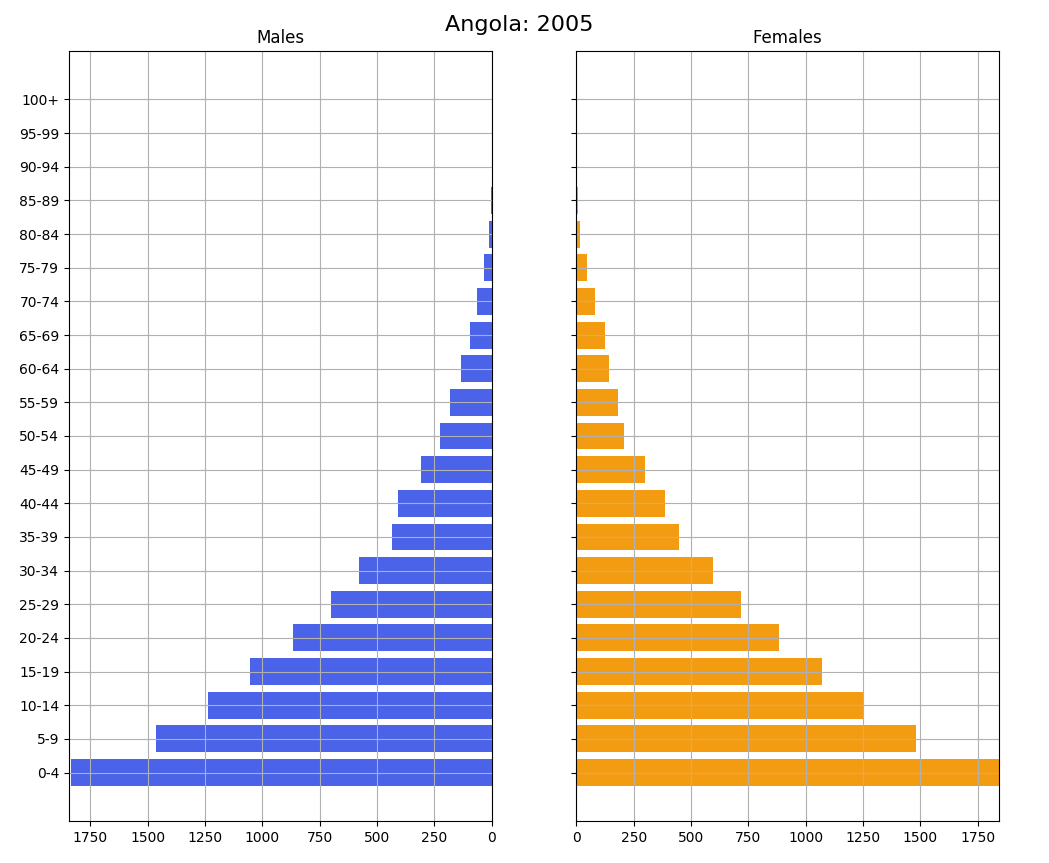
\includegraphics[scale=0.30]{1.png}
\label{fig:2}
\end{figure}

\end{frame}

\begin{frame}{La Pirámide de Edades}

\begin{figure}[hbtp]
\centering
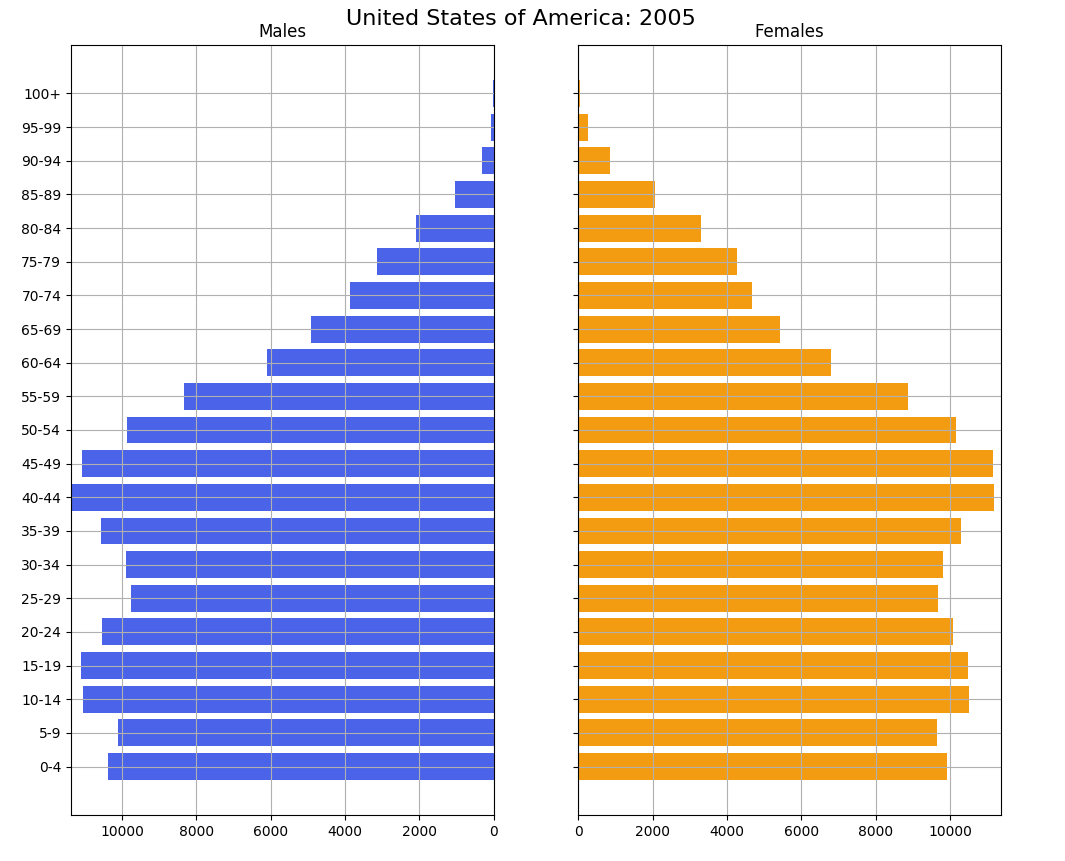
\includegraphics[scale=0.30]{2.png}
\label{fig:3}
\end{figure}

\end{frame}

\begin{frame}{La Pirámide de Edades}

\begin{figure}[hbtp]
\centering
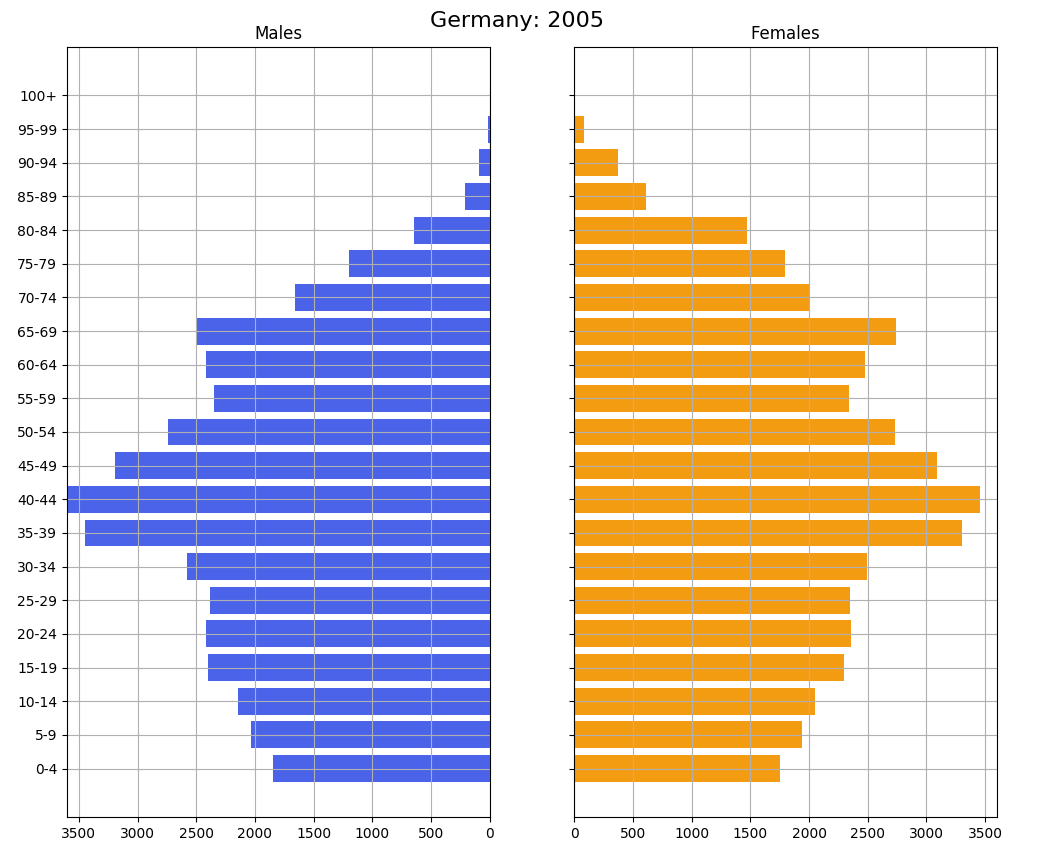
\includegraphics[scale=0.30]{3.png}
\label{fig:4}
\end{figure}

\end{frame}

\begin{frame}{La Pirámide de Edades}

\begin{figure}[hbtp]
\centering
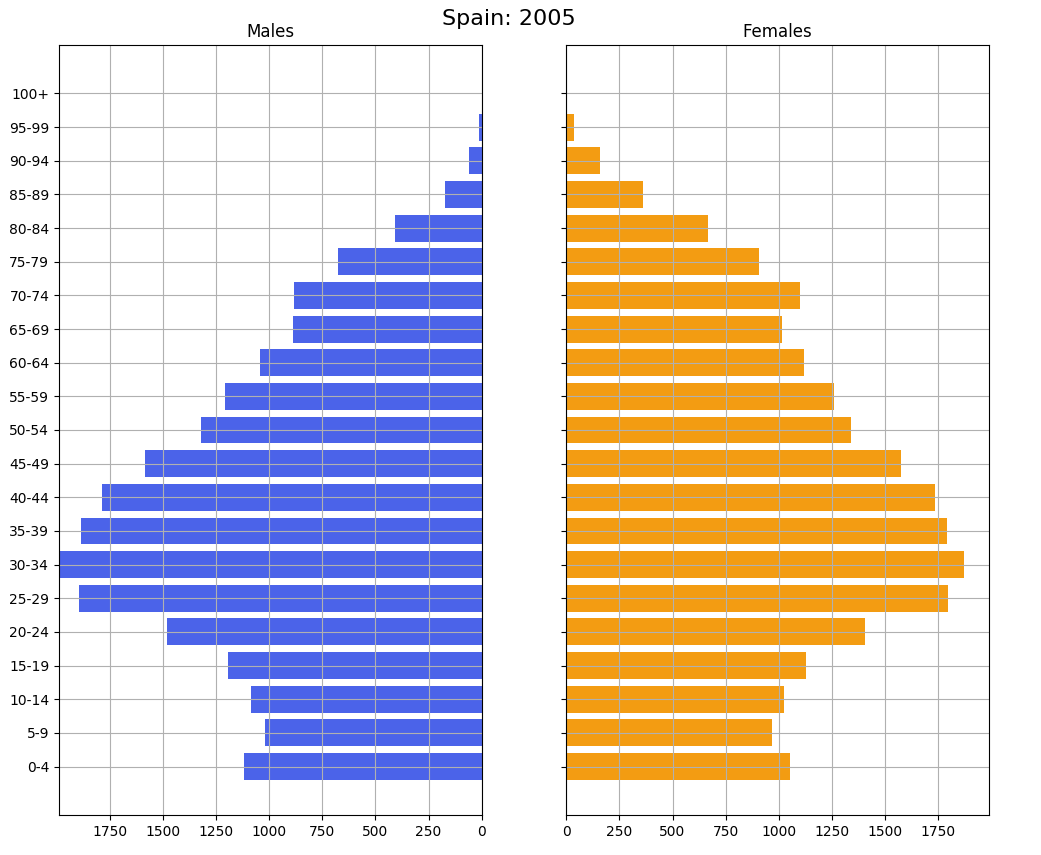
\includegraphics[scale=0.30]{4.png}
\label{fig:5}
\end{figure}

\end{frame}

\begin{frame}{La Pirámide de Edades}

\begin{figure}[hbtp]
\centering
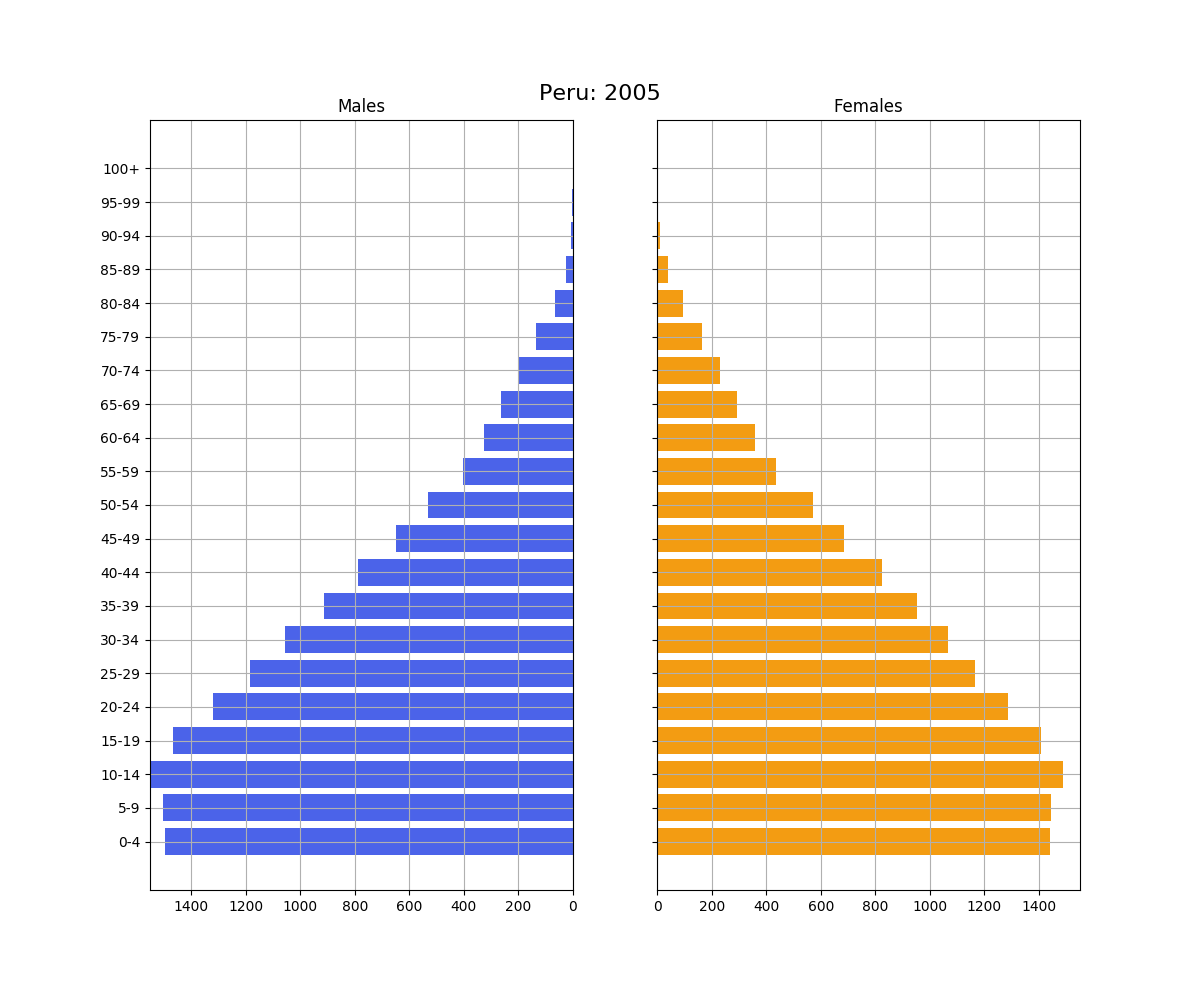
\includegraphics[scale=0.30]{5.png}
\label{fig:6}
\end{figure}

\end{frame}


\begin{frame}{\textbf{Referencias Bibliográficas}}

\begin{itemize}
\justifying
\item Castro Martín, T., \& Domínguez Martín, R. (2007). Las pirámides de población: una aproximación teórico-práctica. Centro de Investigaciones Sociológicas.

\item Castro Martín, T., Domínguez Martín, R., \& Solé-Auró, A. (2011). Las pirámides de población en la demografía española. Revista Española de Investigaciones Sociológicas, 135, 83-116.

\item García Calvente, M. M., \& Alonso Blas, C. (2012). Análisis de las pirámides de población para la planificación sanitaria: propuesta de un modelo de análisis por cohortes de edad y sexos. Gaceta Sanitaria, 26(5), 472-478.

\item Gil-Alonso, F., \& Adiego Sancho, P. (2010). El análisis de las pirámides de población y su aplicación al estudio de la estructura demográfica. Boletín de la Asociación de Geógrafos Españoles, (53), 21-41.

\item Instituto Nacional de Estadística (INE). (2019). Pirámides de población. Recuperado de https://www.ine.es/jaxiT3/Tabla.htm?t=2852

\item Lamas, E., \& Moreno, A. (2008). Pirámides de población y políticas públicas en América Latina. Santiago de Chile: CEPAL.

\item López Roldán, P. (2017). Pirámides de población: una herramienta para el análisis demográfico. Nóesis: Revista de Ciencias Sociales y Humanidades, 26(51), 98-115.
\end{itemize}

\end{frame}

}
\end{document}